\documentclass{standalone}

% ==== Essential Packages ====
\usepackage{tikz}
\usepackage{xcolor}

% ==== Custom Colors ====
\definecolor{softyellow}{HTML}{F2D648}

\begin{document}

\begin{minipage}[t]{0.48\textwidth}
  \centering
  \textbf{\Large{Twistronics}}\\[0.4cm]
  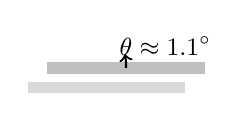
\begin{tikzpicture}[scale=0.5]
    \fill[gray!30] (0,0) -- (4,0) -- (4,0.3) -- (0,0.3) -- cycle;
    \fill[gray!50] (0.5,0.5) -- (4.5,0.5) -- (4.5,0.8) -- (0.5,0.8) -- cycle;
    \draw[thick, ->] (2.5,0.65) arc (0:10:2);
    \node at (3.5,1.2) {\small $\theta \approx 1.1^\circ$};
  \end{tikzpicture}
  \vspace{-0.05cm}

  \begin{itemize}\footnotesize
    \item Multiple layers required
    \item Precise angle control ($\pm 0.1^\circ$)
    \item Complex fabrication
  \end{itemize}
  \begin{equation*}
    \theta_m = 1.1^\circ \Rightarrow \text{Flat bands}
  \end{equation*}
\end{minipage}%
\hfill
\begin{minipage}[t]{0.48\textwidth}
  \centering
  \textbf{\Large{Rippletronics}}\\[0.4cm]
  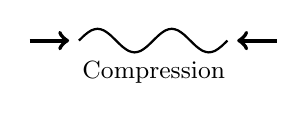
\begin{tikzpicture}[scale=0.5]
    \draw[thick, domain=0:4*pi, smooth, variable=\x]
      plot ({\x*0.3}, {0.3*sin(\x r)});
    \draw[thick, ->, line width=1.5pt] (-1.25,0) -- (-0.25,0);
    \draw[thick, ->, line width=1.5pt] (4.77+0.25,-0) -- (3.77+0.25,0);
    \node at (1.9,-0.8) {\small Compression};
  \end{tikzpicture}
  \vspace{-0.07cm}
  \begin{itemize}\footnotesize
    \item \textbf{\colorbox{softyellow}{Single layer only}}
    \item \textbf{\colorbox{softyellow}{Strain control (continuous)}}
    \item \textbf{\colorbox{softyellow}{Simple implementation}}
  \end{itemize}
  \vspace{-0.08cm}      
  \begin{equation*}
    C > C_{\text{onset}} \Rightarrow \text{Flat bands}
  \end{equation*}
\end{minipage}

\end{document}
